\chapter{Разработка архитектуры}
\label{cha:ch_2}

Для начала декомпозируем задачу. Сначала нужно реализовать:
\begin{enumerate}
    \item Кнопку меню;
    \item Строку статуса;
    \item Счетчик количества открытых браузерных вкладок;
    \item Логотип, который может превращаться в дудл;
    \item Омнибокс с кнопкой камеры;
    \item Информеры погоды, дорожного трафика, почты и чатов;
    \item Вкладки сервисов.
\end{enumerate}

После всего этого нужно будет реализовать анимацию схлопывания Бендера.

Теперь нам нужно разработать базовый макет, расположив все эти элементы на нем.
Для начала заметим, что некоторые элементы можно сгруппировать таким образом,
чтобы получившиеся группы были расположены вертикально друг за другом
(см. рис.~\ref{fig:3-2-vertical}).
Такая группировка позволяет нам использовать в качестве корневого
элемента макета \texttt{LinearLayout} — контейнер,
распологающий элементы подряд вертикально или горизонтально.

\begin{figure}[h]
    \center{\includegraphics[scale=0.333333333]{3-2-vertical}}
    \caption{Визуализация корневого элемента верстки}
    \label{fig:3-2-vertical}
\end{figure}

Сгруппированные вместе кнопку меню, строку местоположения
и счетчик количества браузерных вкладок помещаем
во вложенный \texttt{LinearLayout}, располагая элементы горизонтально
друг относительно друга. С информерами поступаем так же.

Описав такую верстку в xml-файле, мы получаем возможность
во время исполнения приложения создавать дерево объектов,
каждый из которых является экземпляром наследника класса \texttt{View}.
Эти экземпляры отвечают за отображение данных пользователю.

Для каждого из экземпляров нужно будет написать свою логику обновления данных
и реагирования на события, порожденные пользователем.
Чтобы предоставить удобный интерфейс, позволяющий изменять отображаемые данные
и подписываться на события, порождаемые пользователем,
заведем класс \texttt{BenderViewHolder} с набором публичных методов,
обеспечивающих реализацию такой функциональности.
Но не будем реализовывать необходимую
логику непосредственно в самом \texttt{BenderViewHolder},
а заведем для каждого элемента свой класс и будем делегировать
реализацию этим классам (см. рис.~\ref{fig:3-2-hierarchy}).

\begin{figure}[h]
    \center{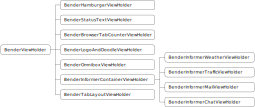
\includegraphics[width=\textwidth]{3-2-hierarchy}}
    \caption{Иерархия классов, реализующих функциональность Бендера}
    \label{fig:3-2-hierarchy}
\end{figure}
